\documentclass[a4paper]{article}
\usepackage[letterpaper, margin=1in]{geometry} % page format
\usepackage{listings} % this package is for including code
\usepackage{graphicx} % this package is for including figures
\usepackage{amsmath}  % this package is for math and matrices
\usepackage{amsfonts} % this package is for math fonts
\usepackage{tikz} % for drawings
\usepackage{hyperref} % for urls
\usepackage{stackengine}
\usepackage[autostyle]{csquotes}

\newcommand\tab[1][0.5cm]{\hspace*{#1}}

\title{Final Exam}
\author{Kaitlyn Mulligan}
\date{5/15/19}

\begin{document}
\lstset{language=Python}

\maketitle

\section{Instructions}
This test could be written in \LaTeX, just as all homework assignments.  Write in understandable, 
easy to follow English.  Make sure you provide good illustrations and figures.  Remember to 
include all your Python programs in your GitHub repository.\\
\tab Your test should be submitted in two ways: through GitHub, and in hard copy (slide it under 
my office's door before the deadline).  Use the \textbf{same} repository you have been using and 
submit your work in a folder named ``\verb|lastname-final|'', where lastname is your last name.

% ----------------------------------------------------------------------------------------------

\section{Problem Set}
The following is a list of problems you will work on.  When providing your solutions (hopefully 
using \LaTeX), do not simply give the final answer, show how you arrived to the solution, justify 
your assumptions, and explain your results clearly.

% ----------------------------------------------------------------------------------------------

\begin{enumerate}
    \item[1.] \textbf{Support Vector Machines}
    \begin{itemize}
        \item[(a)] Download the python program \verb|final.SVM.sinc.py| which implements a 
        10-fold cross-validation approach to find the best set of hyper-parameters $C, \epsilon$ 
        (epsilon), and $\gamma$ (gamma), in an Support Vector Machine for Regression (SVR).

        \textbf{Solution:} I downloaded the python program \verb|final.SVM.sinc.py| as well as 
        uploaded it to my Colab for this final exam.  

        \item[(b)] Download the python program \verb|finalGenData.py| which generates data points 
        of the ``sinc'' function contaminated with random noise.
        
        \textbf{Solution:} I downloaded the python program \verb|finalGenData.py| as well as 
        uploaded it to my Colab for this final exam.  To get an initial idea of the output for 
        this program I ran it using the preset number of samples, $N = 100$.  The results for this 
        showed that the best values for each of the parameters were $C = 0.125, \epsilon = 0.0,$ 
        and $\gamma = 8.0$.  With these values, the program produced a testing set CV score of 
        $-0.270380$.  In addition to these values, it produced the following graph.
        \begin{center}
            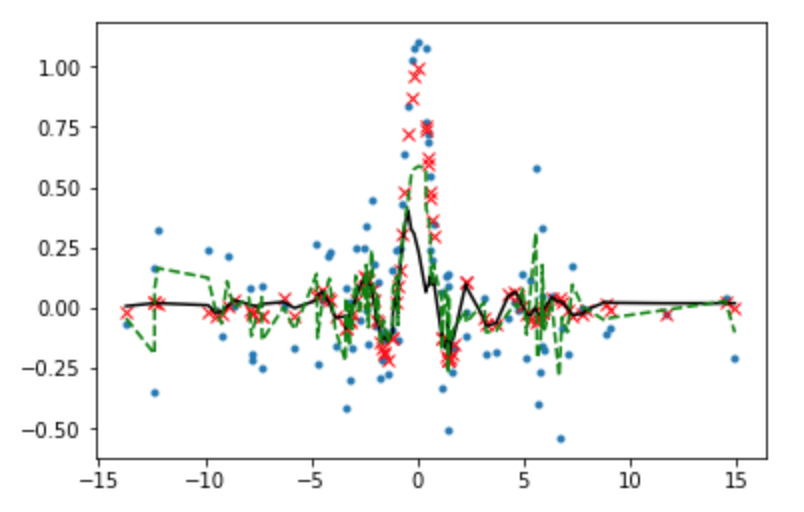
\includegraphics[width=0.6\textwidth]{1b-100-graph.jpg}
        \end{center}

        \item[(c)] Modify the program in 1.(a) to run for 1,000 samples, and then report the best 
        set of hyper-parameters found.  Go here  \verb|https://goo.gl/forms/X1maf8zSIjPhoyNA2| and 
        report your results.  You can do it as many times as you want, but at least one is 
        required.
        
        \textbf{Solution:} Modifying the program in 1.(a), I changed $N = 100$ to $N = 1,000$ so 
        that it will run for 1,000 samples instead of 100.  The best set of hyper-parameters that 
        the program found were $C = 0.125, \epsilon = 0.0,$ and $\gamma = 2.0$.  This produced a 
        testing set CV score of $0.019832$.  It also produced the following graph.
        \begin{center}
            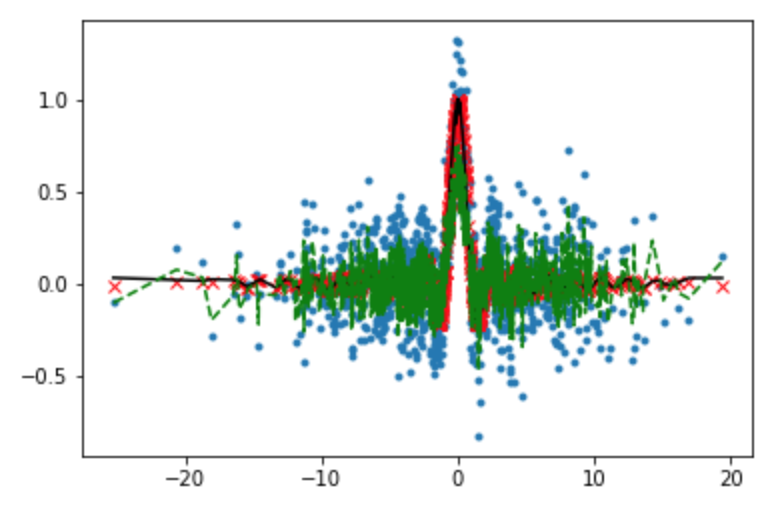
\includegraphics[width=0.6\textwidth]{1c-1000-graph.jpg}
        \end{center}

        \item[(d)] \textbf{Explain} your results.  How do you interpret the hyper-parameters?  
        Is there a great penalty?  Is there room for errors without penalty?  Is there a 
        relationship between $C$ and $\epsilon$?  Any other thoughts?
        
        \textbf{Solution:} While analyzing this graph, note that the blue is the data contaminated 
        with random noise, red represents the actual values, the black are the predicted y values, 
        and the green are the logistic regression predicted values.  Looking at this graph we can 
        see that our prediction did fairly well for the majority of the domain.  Recall, the best 
        set of hyperparameters are $C = 0.125, \epsilon = 0.0,$ and $\gamma = 2.0$.  When looking at 
        the output of the program, we want a higher CV score.  Therefore, we can see that there is 
        a new value printed every time the CV score is higher than the current best.  Thus, this 
        set of hyperparameters has the highest CV score.  Recall, $C$ is the penalty parameter of 
        the error term and $\epsilon$ is the epsilon-tube within which no penalty is associated.  
        The penalty is not huge, but also not small.  As we can see, $\epsilon$ is 0.0, therefore 
        there is no room for errors without penalty.  I believe there is a relationship between 
        $C$ and $\epsilon$ because $C$ explains trade off between the complexity of the model and 
        the degree to which the deviations are larger than the $\epsilon$ allowed.  The values of 
        $C$ and $\epsilon$ are both important because the bigger or smaller the value of $\epsilon$ 
        affects how many support vectors are selected.  Thus, $C$ and $\epsilon$ relate to the model 
        complexity but in different ways.

        \item[(e)] (\textbf{Extra credit} +10) Repeat 1.(c)-(d) but for 10,000 samples.
         
        \textbf{Solution:} Modifying the program to run for 10,000 samples, I changed $N = 1,000$ 
        to $N = 10,000$ so that it will run for 10,000 samples instead of 1,000.  This program took 
        a very long time and did not finish running after 12 hours.  After 12 hours, Google Colab 
        runtime disconnected and I did not obtain final results.  The best values for the 
        hyperparameters that I obtained before it disconnected were $C = 0.125, \epsilon = 0.0,$ and 
        $\gamma = 2.0$.  With these values, the program produced a testing set CV score of $0.274826$.  
        Since the runtime disconnected, I was unable to obtain a graph.  Recall, $C$ is the penalty 
        parameter of the error term and $\epsilon$ is the epsilon-tube within which no penalty is 
        associated.  The penalty is not huge, but also not small.  As we can see, $\epsilon$ is 0.0, 
        therefore there is no room for errors without penalty.
    \end{itemize} 


% ----------------------------------------------------------------------------------------------
    
    \item[2.] \textbf{More Support Vector Machines}.  For this part you will use the digits 
    dataset.  For reading the dataset, you should use the following Python code in a file named 
    \verb|finalGetDigits.py|:
    \lstinputlisting[language=Python,frame=single]{finalGetDigits.py}
    Once saved do the following:
    \begin{itemize}
        \item[(a)] Download the python program \verb|final.SVM.dig.py| which implements a 10-fold 
        cross-validation approach to find the best set of hyper-parameters $C, \epsilon$ (epsilon), 
        and $\gamma$ (gamma), in an Support Vector Machine for Regression (SVR) in the digits 
        dataset.

        \textbf{Solution:} After saving \verb|finalGetDigits.py|, I downloaded the python program 
        \verb|final.SVM.dig.py| as well as uploaded it to my Colab for this final exam.

        \item[(b)] Run the program in 2.(a) and modify it if you need to, to find and report the 
        best set of hyper-parameters and the final validation score.  Save the plot and interpret 
        it, give your comments about it.
        
        \textbf{Solution:} After running the program, I obtained that the hyperparameters were $C = 
        4096.0, \epsilon = 1.7,$ and $\gamma = 0.03125$.  This produced a testing set CV score of 
        $0.335940$.  The graph below was produced from this program.  The colormap is based on a 
        spectrum of colors depending on the value of \verb|ypred|. The numbers represented on the 
        graph are the target outputs of \verb|y|.
        \begin{center}
            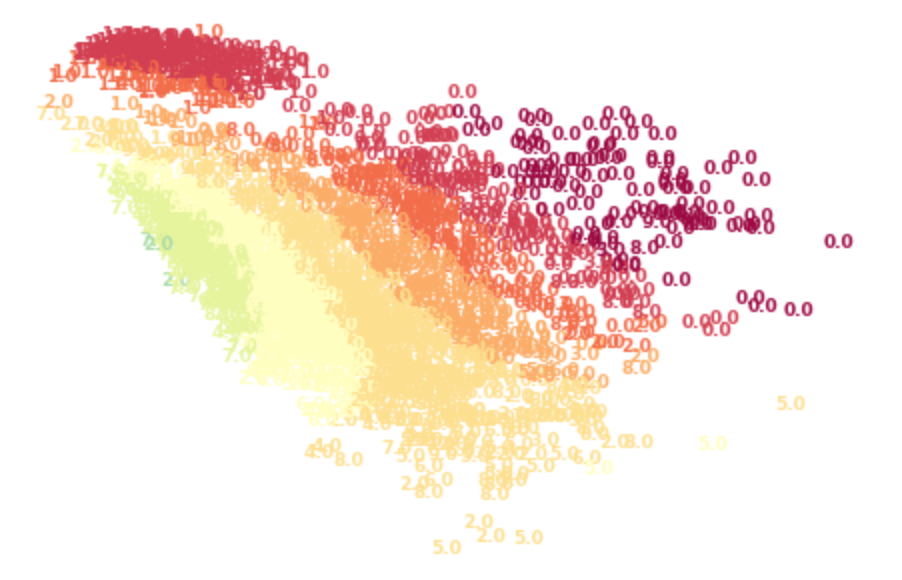
\includegraphics[width=0.6\textwidth]{2b-graph.jpg}
        \end{center}

        \item[(c)] \textbf{Explain} your results.  How do you interpret the hyper-parameters?  
        Is there a great penalty?  Is there room for errors without penalty?  Is there a 
        relationship between $C$ and $\epsilon$?  Any other thoughts?
        
        \textbf{Solution:} Recall, the numbers represented in the graph are the target outputs of 
        \verb|y|.  Also the colormap is based on a spectrum of colors depending on the value of 
        \verb|ypred|.  The best set of hyperparameters obtained from this program were $C = 4096.0, 
        \epsilon = 1.7,$ and $\gamma = 0.03125$.  This produced a testing set CV score of $0.335940$.
        Recall, $C$ is the penalty parameter of the error term and $\epsilon$ is the epsilon-tube 
        within which no penalty is associated.  Here we have that the penalty of the error is very 
        large.  Also, with $\epsilon = 1.7$, we have that there is some room for errors without penalty.  
        I believe that there is a relationship between $C$ and $\epsilon$ because $C$ explains the trade 
        off between the complexity of the model and the degree to which the deviations are larger than 
        the $\epsilon$ allowed.  Both of these values are important as they both impact how many support 
        vectors will be selected.
        
        \item[(d)] (\textbf{Extra credit} +30) Prepare and share a single Colaboratory for both 
        1.(c)-(d) and 2.(b)-(c).  You should use proper headings and comments and explanations.  
        \textit{Pro Tip:} you may have to combine all files into a single program or upload files 
        on demand.

        \textbf{Solution:} I have prepared a single Colaboratory for both 1.(c)-(d) and 2.(b)-(c).  
        There are headings for each section labeling what everything is.  Below is a link to the Colab 
        I created.  In addition, I have uploaded the notebook to GitHub.\\
        \verb|https://colab.research.google.com/drive/1BjQQwIJypzanJwk8sSEXQBpCknTfxkRt|.
    \end{itemize}
\end{enumerate}

\end{document}
